%presentation in Beamer

\documentclass{beamer}

\usepackage{amsmath}
\usetheme{default}

\title[OIL!]{OIL! OR WILL THERE?}
\subtitle[Errors]{The Decline of Norwegian Oil}
\author[J. Mauritzen]{Johannes Mauritzen}
\institute[NHH]{
  Department of Business and Management Science\\
  NHH Norwegian School of Economics\\[1ex]
  \texttt{johannes.mauritzen@nhh.edu}
}
\date[Oct 2013]{October 2013}

\begin{document}

%--- the titlepage frame -------------------------%
\begin{frame}[plain]
  \titlepage
\end{frame}


%--- the presentation begins here ----------------%

%--- Intro 						  ----------------%
%--- the presentation begins here ----------------%

\begin{frame}[plain]
	\begin{figure}
	\includegraphics[width=.5\textwidth]{sinclair.png}
	\end{figure}
\end{frame}


\begin{frame}[plain]
	\begin{figure}
	\includegraphics[width=.5\textwidth]{there_will_be_blood_ver4.jpg}
	\end{figure}
\end{frame}

%--- the presentation begins here ----------------%

\begin{frame}[plain]
	\begin{figure}
	\includegraphics[width=1\textwidth]{oil_decline.png}
	\end{figure}
\end{frame}

%--- alternate titles----------------%

\begin{frame}[plain]
or...\\
Naive Modeling of Oil Field Data
\end{frame}

\begin{frame}[plain]
or...\\
Naive Modeling of Oil Field Data\\[1cm]
or...\\
A top-down-bottom-up multilevel non-parametric generalized additive model of oil field production in the Norwegian continental shelf\\
\end{frame}

\begin{frame}[plain]
or...\\
Naive Modeling of Oil Field Data\\[1cm]
or...\\
A top-dow-bottom-up multilevel non-parametric generalized additive model of oil field production in the Norwegian continental shelf\\[1cm]
or...\\
Oil Price Does Not Seem to Matter (Much) for Production in Existing Fields\\
\end{frame}

%--- the presentation begins here ----------------%

\begin{frame}[plain]
	\begin{figure}
	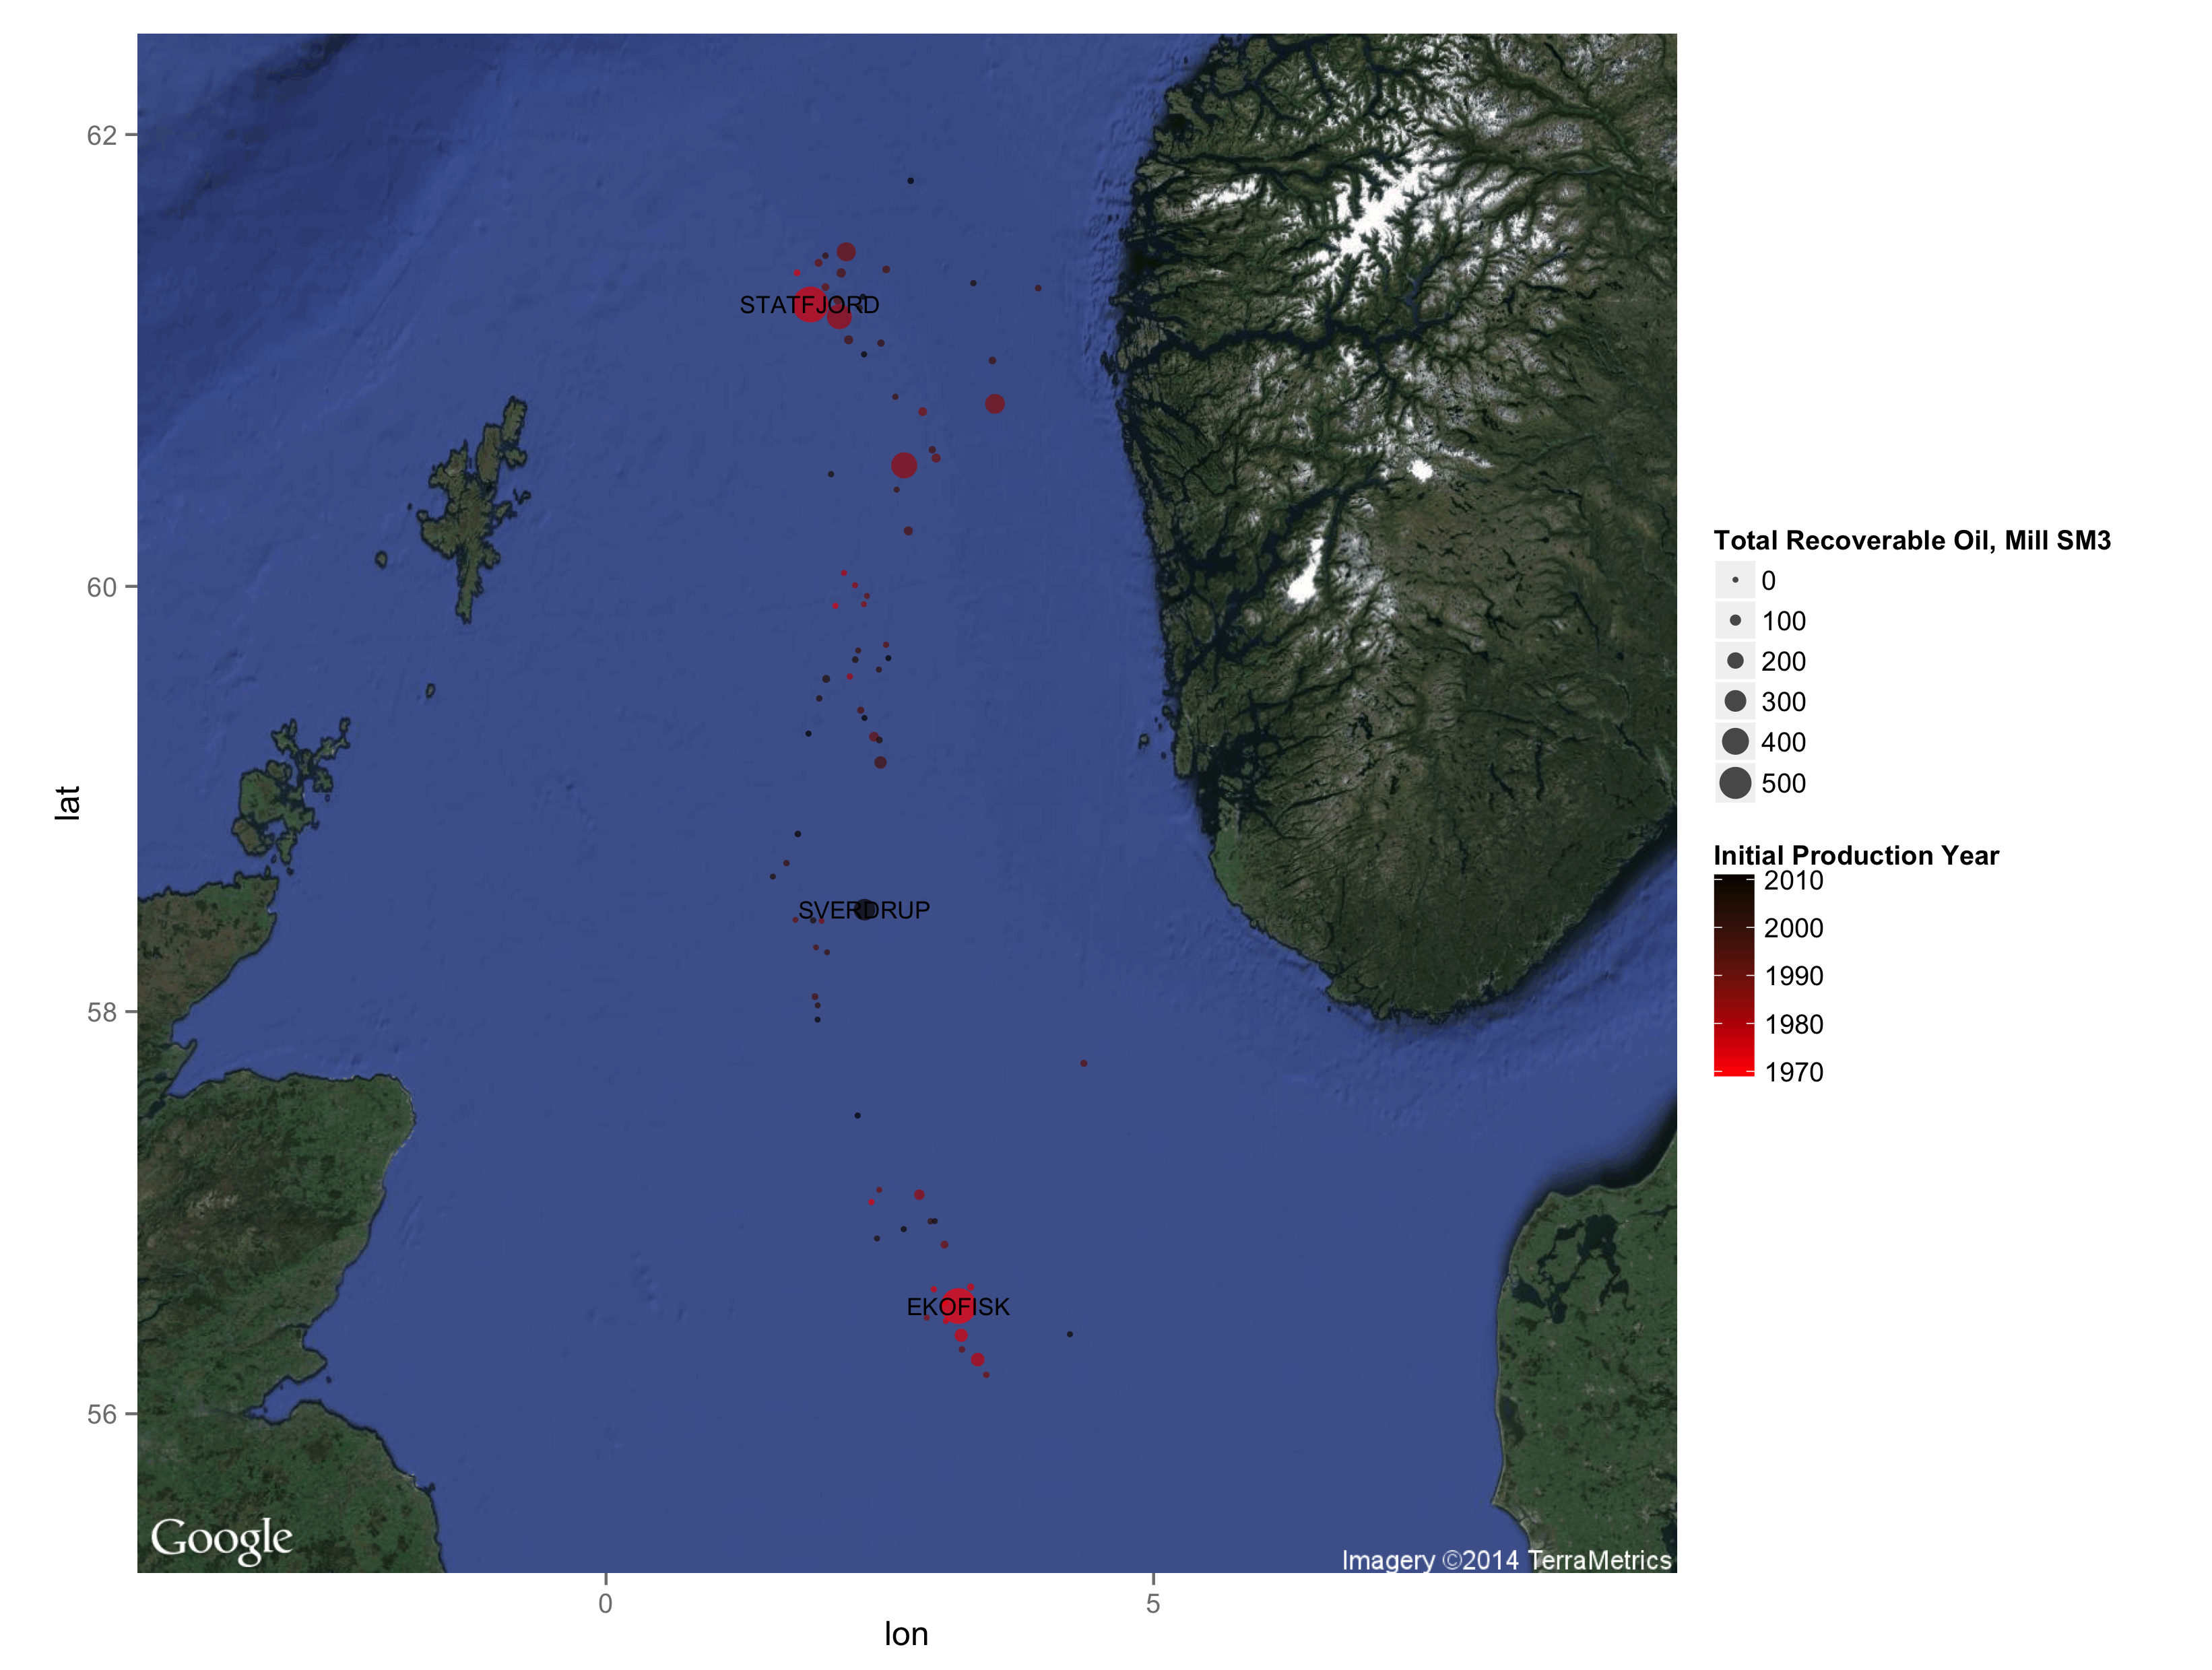
\includegraphics[width=1\textwidth]{north_sea_reserves.png}
	\end{figure}
\end{frame}

%--- the presentation begins here ----------------%

\begin{frame}[plain]
	\begin{figure}
	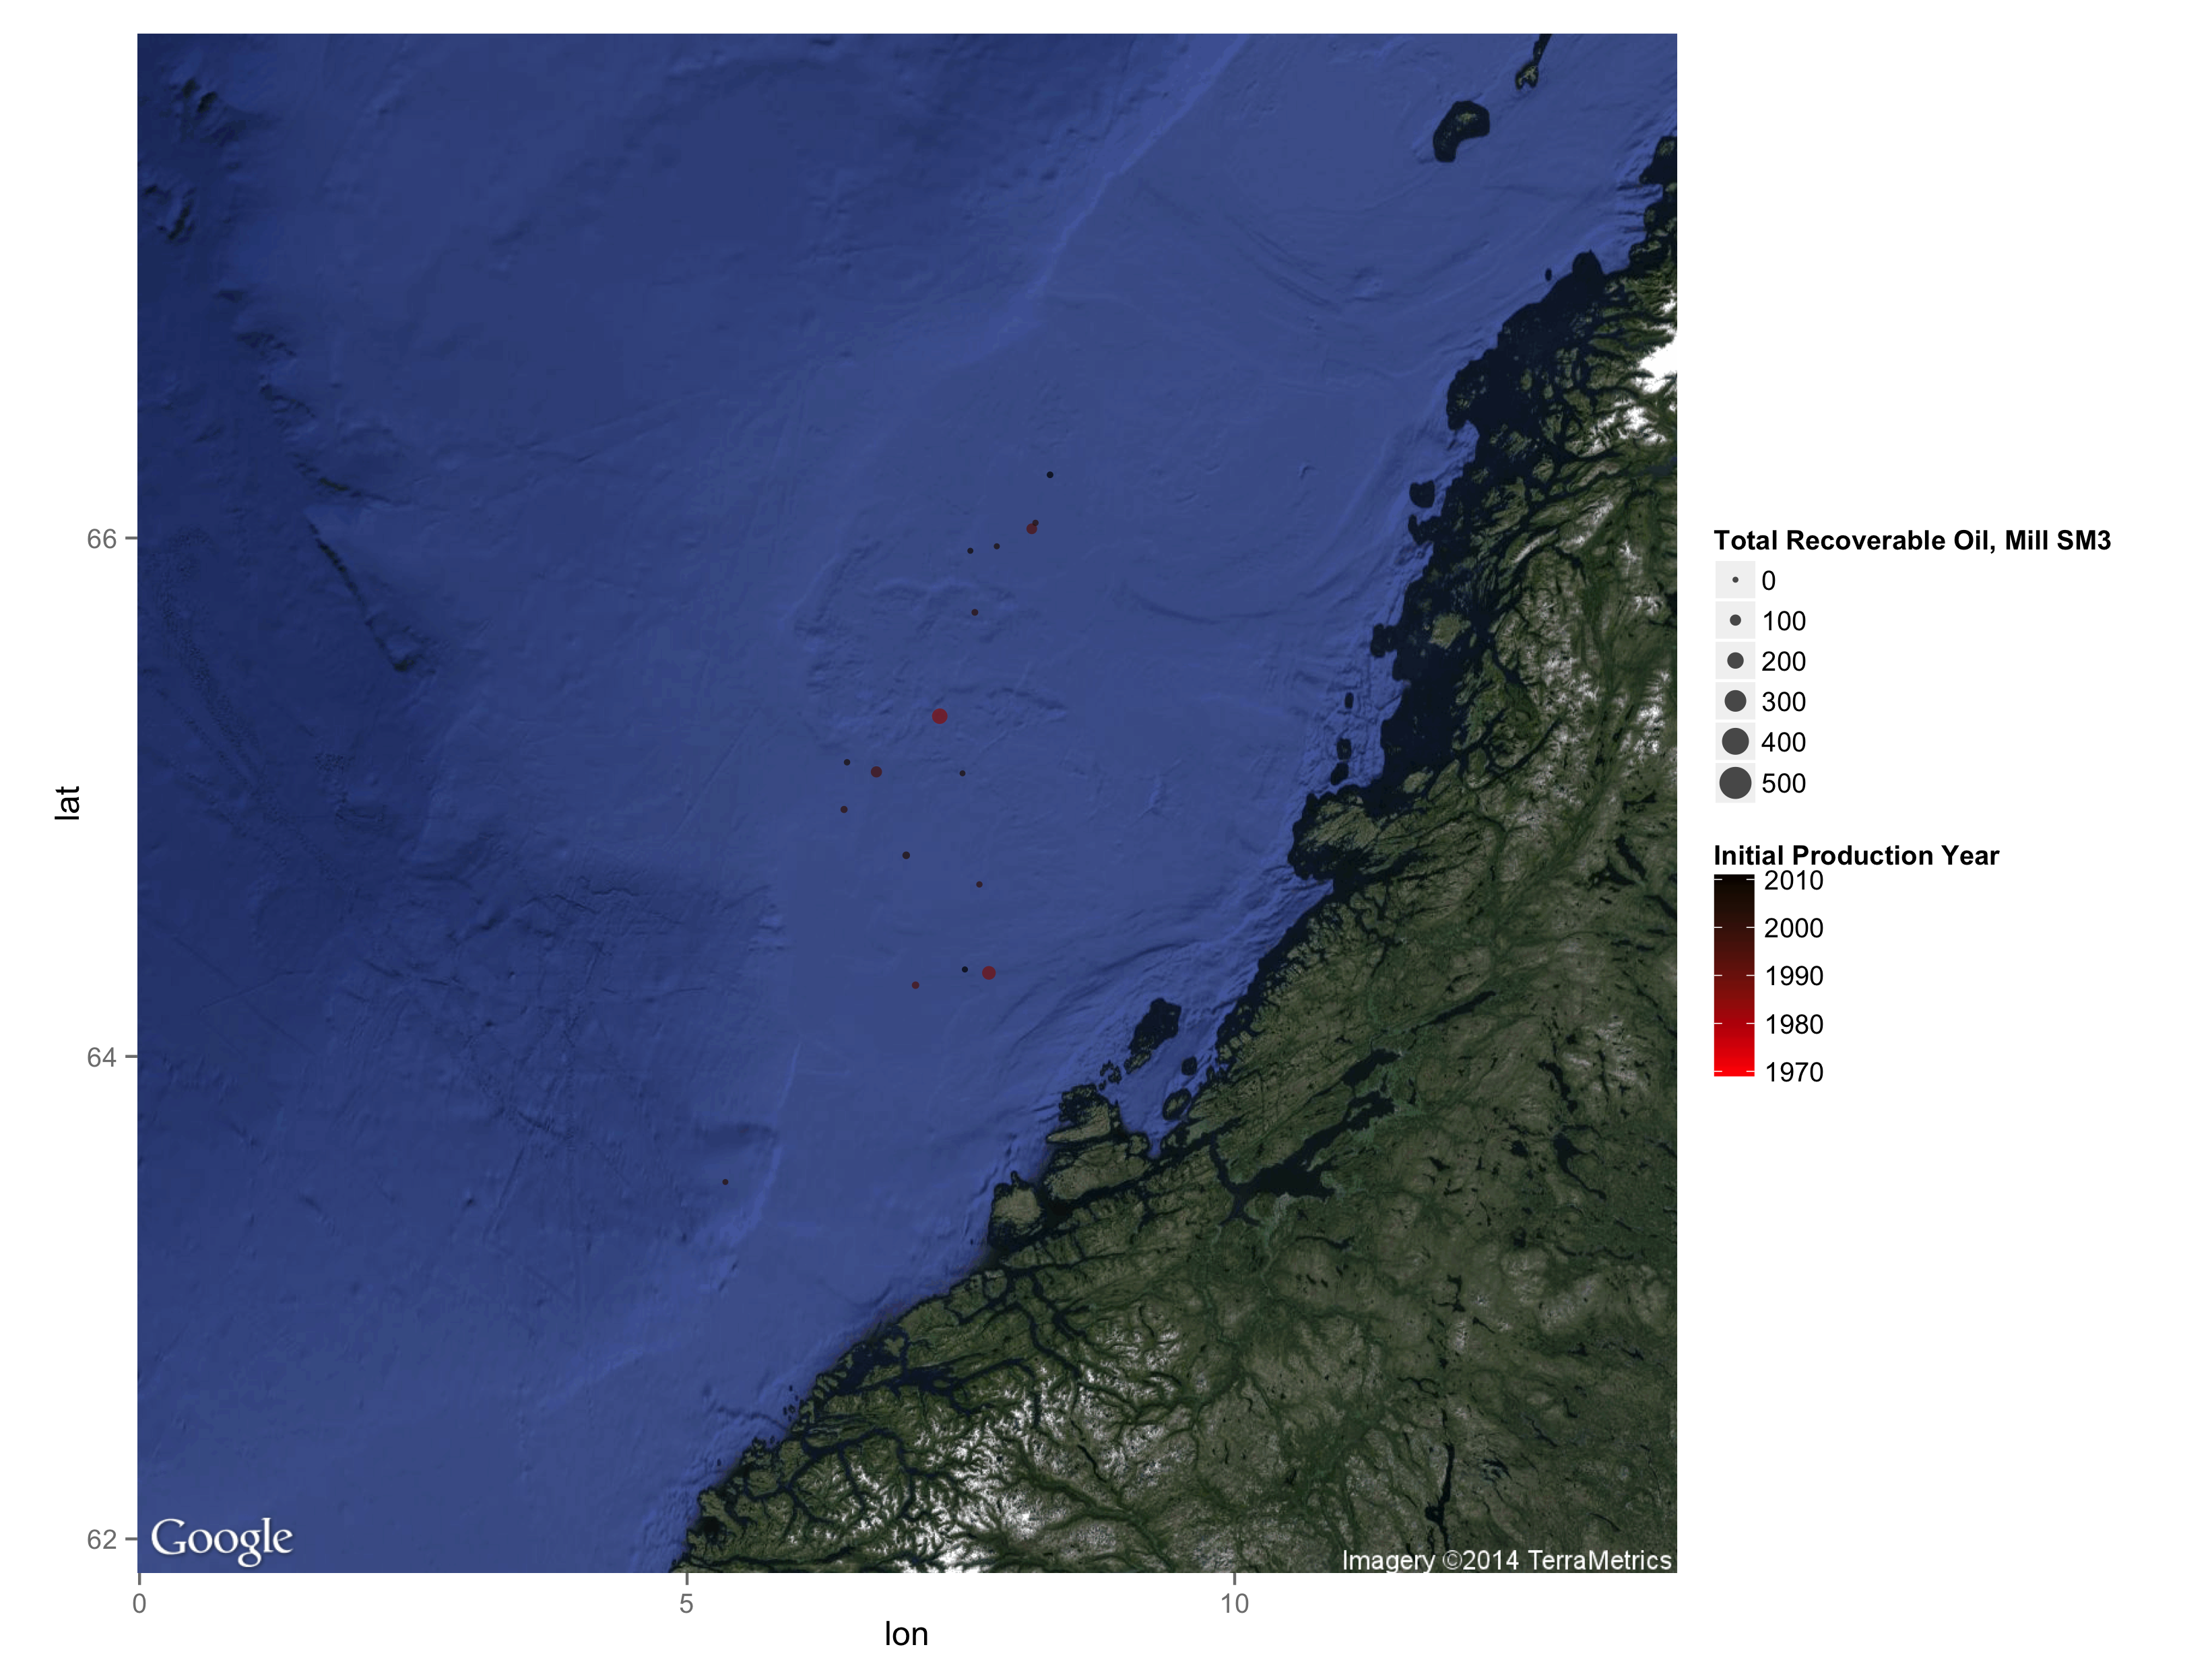
\includegraphics[width=1\textwidth]{norwegian_sea_reserves.png}
	\end{figure}
\end{frame}

%--- the presentation begins here ----------------%

\begin{frame}[plain]
	\begin{figure}
	\includegraphics[width=1\textwidth]{tot_exist_prod_cf.png}
	\end{figure}
\end{frame}


%--- Investment ----------------%

\begin{frame}[plain]
	\begin{figure}
	\includegraphics[width=1\textwidth]{invest_with_oil_price.png}
	\end{figure}
\end{frame}

%--- the presentation begins here ----------------%

\begin{frame}[plain]
	\begin{figure}
	\includegraphics[width=1\textwidth]{size_vs_init_prod.png}
	\end{figure}
\end{frame}

%--- the presentation begins here ----------------%

\begin{frame}[plain]
	\begin{figure}
	\includegraphics[width=1\textwidth]{invest_per_prod.png}
	\end{figure}
\end{frame}

%--- the presentation begins here ----------------%

\begin{frame}[plain]
	\begin{figure}
	\includegraphics[width=1\textwidth]{invest_per_prod_l5.png}
	\end{figure}
\end{frame}


%--- naive GLM formula and results ----------------%
\begin{frame}[plain]
	\begin{multline}
	\nonumber  Log(Production_{i,t})=\alpha_0 + \alpha_1 time\_to\_peak_{i,t} + \alpha_2 time\_to\_peak_{i,t}^2 \\
	 + \alpha_3 time\_to\_peak_{i,t}^3  + \alpha_4 peak\_to\_end_{i,t} + \alpha_5 peak\_to\_end_{i,t}^2 \\
	 + \alpha_6 peak\_to\_end_{i,t}^3 + \gamma total\_recoverable\_oil_i \\
	 + \beta_1 oil\_price + \beta_2 oil\_price\_l1 + ...+ \epsilon
	\end{multline}
\end{frame}


\begin{frame}[plain]
	\begin{figure}
	\includegraphics[width=1\textwidth]{glm_dirty_box.png}
	\end{figure}
\end{frame}

\begin{frame}[plain]
	\begin{figure}
	\includegraphics[width=1\textwidth]{oil_decline.png}
	\end{figure}
\end{frame}

%--- Show Example of a Simple GAM ----------------%


\begin{frame}[plain]
	\begin{figure}
	\includegraphics[width=1\textwidth]{statfjord_plot.png}
	\end{figure}
\end{frame}


\begin{frame}[plain]
	\begin{multline}
	\nonumber Production_{statfjord,t}=f(time) + \epsilon
	\end{multline}
\end{frame}


\begin{frame}[plain]
	\begin{figure}
	\includegraphics[width=1\textwidth]{statfjord_gam.png}
	\end{figure}
\end{frame}

%--- as well as on ekofisk ----------------%
\begin{frame}[plain]
	\begin{figure}
	\includegraphics[width=1\textwidth]{ekofisk_plot.png}
	\end{figure}
\end{frame}

%--- Benchmark modelling formula ----------------%
\begin{frame}[plain]
	\begin{multline}
	\nonumber Log(Production_{i,t})=f(time\_to\_peak_{i,t}, total\_recoverable\_oil_i) \\
	+ f(peak\_to\_end_{i,t}, total\_recoverable\_oil_i)
	+ f(year_{i,t}) + \epsilon
	\end{multline}

	\begin{equation}
		\nonumber \epsilon \sim Normal(0, \sigma^2)
		\end{equation}
\end{frame}
%--- results from modelling ----------------%

\begin{frame}[plain]
	\begin{figure}
	\includegraphics[width=1\textwidth]{bench_vs_split.png}
	\end{figure}
	
\end{frame}

%--- modelling formula for price ----------------%
\begin{frame}[plain]
		\begin{multline}
	\nonumber Log(Production_{i,t})=f(time\_to\_peak_{i,t}, total\_recoverable\_oil_i) \\
	+ f(peak\_to\_end_{i,t}, total\_recoverable\_oil_i) \\
	+ \beta_1 oil\_price + \beta_2 oil\_price\_l1 + ... +  \epsilon
	\end{multline}

		\begin{equation}
		\nonumber \epsilon \sim Normal(0, \sigma^2)
		\end{equation}
\end{frame}

%--- results from modelling ----------------%
\begin{frame}[plain]
	\begin{figure}
	\includegraphics[width=1\textwidth]{bench_vs_price.png}
	\end{figure}
\end{frame}

%--- modelling formula for non-price vs. price ----------------%
\begin{frame}[plain]
		\begin{multline}
	\nonumber Log(Production_{i,t})=f(time\_to\_peak_{i,t}) + f(peak\_to\_end_{i,t}) \\
	+ f(total\_recoverable\_oil_i) +  \epsilon
	\end{multline}

		\begin{equation}
		\nonumber \epsilon \sim Normal(0, \sigma^2)
		\end{equation}
\end{frame}
%--- results from modelling ----------------%
\begin{frame}[plain]
	\begin{figure}
	\includegraphics[width=1\textwidth]{price_vs_non_price.png}
	\end{figure}
\end{frame}

\begin{frame}[plain]
	\begin{figure}
	\includegraphics[width=1\textwidth]{coeff_split_plot.png}
	\end{figure}
\end{frame}

%--- Forecasting ----------------%

\begin{frame}[plain]
	\begin{figure}
	\includegraphics[width=1\textwidth]{field_lev_forecast.png}
	\end{figure}
\end{frame}

\begin{frame}[plain]
	\begin{figure}
	\includegraphics[width=1\textwidth]{tot_forecast.png}
	\end{figure}
\end{frame}

\end{document}